 \chapter{Motivation}



% https://www.princeton.edu/news/2016/10/04/good-day-great-ideas-princetons-haldane-wins-one-theoretical-physics
% https://www.aps.org/publications/apsnews/201611/nobel.cfm
% https://www.nobelprize.org/prizes/physics/2016/haldane/biographical/


In 2001 Alexei Yu. Kitaev presented a toy model for implementing qubits
that could face the problem of high decoherency in quantum computation \citep{kitaev_unpaired_2001}. Kitaev's idea was centered in using the properties of an exotic quasi-particle that appears at the edges of a quantum superconducting chain. This quasi-particle receives the name of Majorana Fermion, is characterized for being its own anti-particle, thus it has no charge or spin. It also presents non-Abelian statistics, a desired property to implement fault-tolerant quantum computers\citep{kitaev_fault-tolerant_2003}. These majorana fermions where theoretically predicted since the 1930's by one of the genius of the era, Ettore Majorana \citep{wilczek_majorana_2009}.
Although no fundamental Majorana-particle has been discovered to the
date, Kitaev's model inspired the pursue of majorana fermions as
quasi-particles in a novel exotic class of materials known as topological
superconductors (TS)\citep{fu_superconducting_2008,sato_non-abelian_2009,alicea_new_2012}.
\\

The last five years have been full of excitement, as new experiments
have turned some of the theoretical predictions of the 1990s and 2000s
into a reality. Very recently the first evidence of Majorana end states
in TS has been found in multiple experiments \citep{mourik_signatures_2012,das_zero-bias_2012,deng_anomalous_2012}
following the prescription by \citet{oreg_helical_2010} and \citet{lutchyn_majorana_2010}.
These experiments have been based on tunneling spectroscopy in junctions
between TS and non metallic (NM) leads, where resonances have been
observed at zero energy, consistent with the presence of Majorana
zero\textendash energy modes.\\

A downside of the tunneling spectroscopy technique in this case, is
that it probes not only the end of the Topological Superconductor(TS), but its bulk as well ,
which completely destroys the qubit information. A less destroying
model presented by \citet{liu_detecting_2011} consists consists in attaching a Quantum Dot (QD) to the edges of a majorana chain in the topological phase and executing transport measurements through the QD \cite{liu_detecting_2011} . The majorana mode at the end of the chain then leaks inside the QD \cite{vernek_subtle_2014} which produces a zero-bias conductance peak of half a quanta $\frac{e^{2}}{2h}$ through the dot. This is a majorana signature which produces half of the expected peak by a regular fermion.\\

In fact, this phenomenon is similar to the $\frac{e^{2}}{h}$ conductance peak caused by the Kondo effect \citep{hewson_kondo_1997}. Since topological superconductors and the Kondo effect could coexist at temperatures of a few mili-kelvins, it should be possible to observe combined Kondo-Majorana physics in this type of devices. This idea motivated an NRG study of a Quantum dot-Majorana hibrid system in the Kondo regime  \citep{ruiz-tijerina_interaction_2015}. \\

\begin{figure}[t]
    \centering
    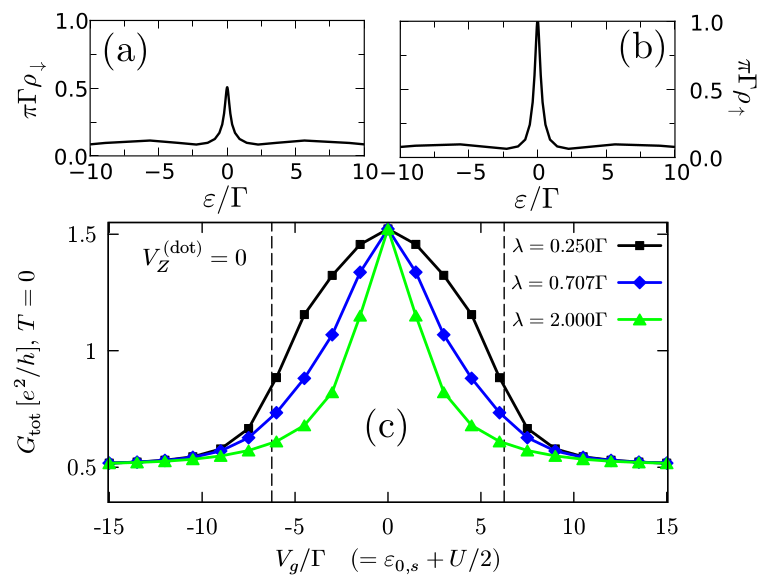
\includegraphics[scale=0.4]{IMAGES/Kondo-MajoranaCond.png}
    \caption{\label{Fig-Kondo-Majorana conductance}(a) QD spin-down
    density of states. Because this channel couples to the Majorana mode,
    it displays the characteristic zero-bias signature of amplitude
    $\frac{e^{2}}{2h}$. (b) QD spin-up density of states,
    displaying the zero-bias peak of the Kondo effect, with
    unit amplitude. (c) Zero-bias conductance of the QD coupled
    to the Majorana mode, as a function of the QD energy level ($\lambda$
    parameterizes the strength of the Majorana-QD tunnel coupling).
    The presence of the spin-up Kondo resonance enhances the
    QD conductance in particle-hole symmetry ($V_{g}=0$),
    but quickly disappears as the QD level is detuned from this point.
    The spin-down Majorana signature, on the other hand, is
    robust {[}7{]}, leaving a residual conductance of $\frac{e^{2}}{2h}$.
    \protect\Source{\citep{ruiz-tijerina_interaction_2015}}.}
\end{figure}

This study revealed that transport measurements
through the quantum dot will show contributions to the enhanced conductance
coming from the Kondo effect and the Majorana mode: The Majorana mode
at the end of the wire will migrate into one of the quantum dot spin channels,
giving rise to a zero\textendash energy peak in the density of states
(\ref{Fig-Kondo-Majorana conductance}a)) contributing a conductance
of $\frac{e^{2}}{2h}$(\ref{Fig-Kondo-Majorana conductance}c)). The
zero\textendash bias peak from the Kondo effect appears in the other
spin channel (\ref{Fig-Kondo-Majorana conductance}b)), contributing
a conductance of $\frac{e^{2}}{h}$. Then, the Kondo effect can be
\textquotedblleft turned off\textquotedblright{} through gate voltages
and magnetic fields, leaving only the Majorana contribution. Clear
evidence of the destruction of the Kondo peak will appear in the conductance,
allowing for a distinction between Majorana and Kondo signatures.\\



 Apart from not destroying the entire qubit-information the QD-method has another insight.  This is the possibility of manipulating  Majorana fermions  in multidot systems by shifting the QD gate voltages and tunnel couplings which brings possible applications in  braiding procedures. The simplest system where Majorana manipulation is possible is  a  Double Quantum Dot (DQD) coupled to a majorana chain. By tuning the QD gate voltages and the majorana coupling we will be able to probe the mobility of the majorana modes through the dots. \\
 
In addition, when both dots are coupled to the lead the Double Quantum Dot exhibits an anti-ferromagnetic interaction known as  Ruderman-Kittel-Kasuya-Yosida (RKKY) \cite{ruderman_indirect_1954,kasuya_theory_1956,yosida_magnetic_1957}. On the other hand, when only one dot is coupled  and the second Dot is indirectly attached through the first dot,  the Kondo effect is annihilated due to the destructive interference  generated by extra dot \cite{dias_da_silva_transmission_2008}. Both cases reveal interesting results for majorana manipulation and hybrid Kondo-Majorana systems.


\section{Structure}

This thesis is integrated by $4$-major chapters . In  \ref{chap:Preliminaries}, we will take a review to the basis of quantum transport in single electron transistors, the Anderson model and the emergence of the Kondo effect in quantum dots. 

In \ref{chap: Methods} contains a description of the methods that we will use to study the Double Quantum Dot-majorana system. The  methods  are the Zubarev's ballistic transport\cite{zubarev_double-time_1960} for non-interacting systems and Wilson's Numerical Renormalization
Group (NRG) technique \citep{wilson_renormalization_1975} for interacting systems. We will use the Double Quantum Dot case as major example to explain both methods. Hence the background information about double quantum dots systems will be presented in this chapter. 

The \ref{chap:Majorana} changes the subject, leading us to the mean topic of this thesis, Majorana fermions. The discussion will start with the Kitaev chain addressing its main characteristics such as topological characterization and non-abelian statistics . Then we take a look to the real implementations of majorana chains were we will discuss the most recent experimental accomplishments  in the area.  At the end, we face the the problem of a hybrid Quantum Dot-Majorana system using the methods described in \ref{chap: Methods}.

Using the methods from \ref{chap: Methods} and the previous acquired experience with the Double Quantum Dot and the Quantum Dot-Majorana , we address in \ref{chap:Results} the  Double Quantum Dot-Majorana system. We will study several procedures  mainly focused in the manipulation of majorana fermions and the combined effects of Kondo-Majorana physics. 







